\section{Experimental Paradigm}
\label{sec:experimental_paradigm}
We first set out to model the infant learning tasks described in
\citet{Smith2002} using simple neural networks. In order to do so, we use
artificial toy data that is designed to mimic the training data described in
the paper. Each object sample is assigned a shape, texture and color value.
There are two types of model evaluations performed, both drawn from
\cite{Smith2002}.

{\bf1. First-order generalization test}: For the first-order generalization
test, infants are asked to evaluate novel instances of familiar objects. To
simulate this test, we train our neural network models to classify objects,
ensuring that objects of the same category are assigned the same shape. Then,
we build a test set by creating one novel exemplar of each category that
appeared in the training set. The novel exemplar has the same shape as the
training exemplars of that category, but a new color and texture combination.
Accuracy is defined as the fraction of test images that are correctly
classified by the model. This test is repeated for different training set
sizes, i.e. different combinations of \{\textit{\# categories},
\textit{\# exemplars}\}. It is important to note that as \textit{\# categories}
increases, the first-order task becomes more difficult.

{\bf2. Second-order generalization test}: For the second-order generalization
test, infants are presented with an exemplar of a novel object category as a
baseline. Then, they are shown 3 comparison objects: one which has the same
shape as the baseline, one with the same color, and one with the same texture.
In each case, the other 2 features are different from the baseline. The infants
are asked to select which of the 3 comparison objects are of the same category
as the baseline object. We simulate this test by creating an evaluation set
containing groupings of 4 samples: the baseline, the shape constant, the color
constant, and the texture constant. Each grouping serves as one test example.
We find which of the 3 samples the NN thinks to be most similar by evaluating
the cosine similarity using the hidden layer features of the model. Accuracy is
defined as the fraction of groupings for which the model chose the correct
(shape-similar) object. This test was repeated for different training set
sizes, i.e. different combinations of \{\textit{\# categories},
\textit{\# exemplars}\}.

\begin{figure*}[h]
    \begin{center}
        % mlp results
        \begin{subfigure}[b]{0.47\textwidth}
            \begin{center}
                % subfigure (a)
                \begin{subfigure}[b]{0.48\textwidth}
                    \begin{center}
                        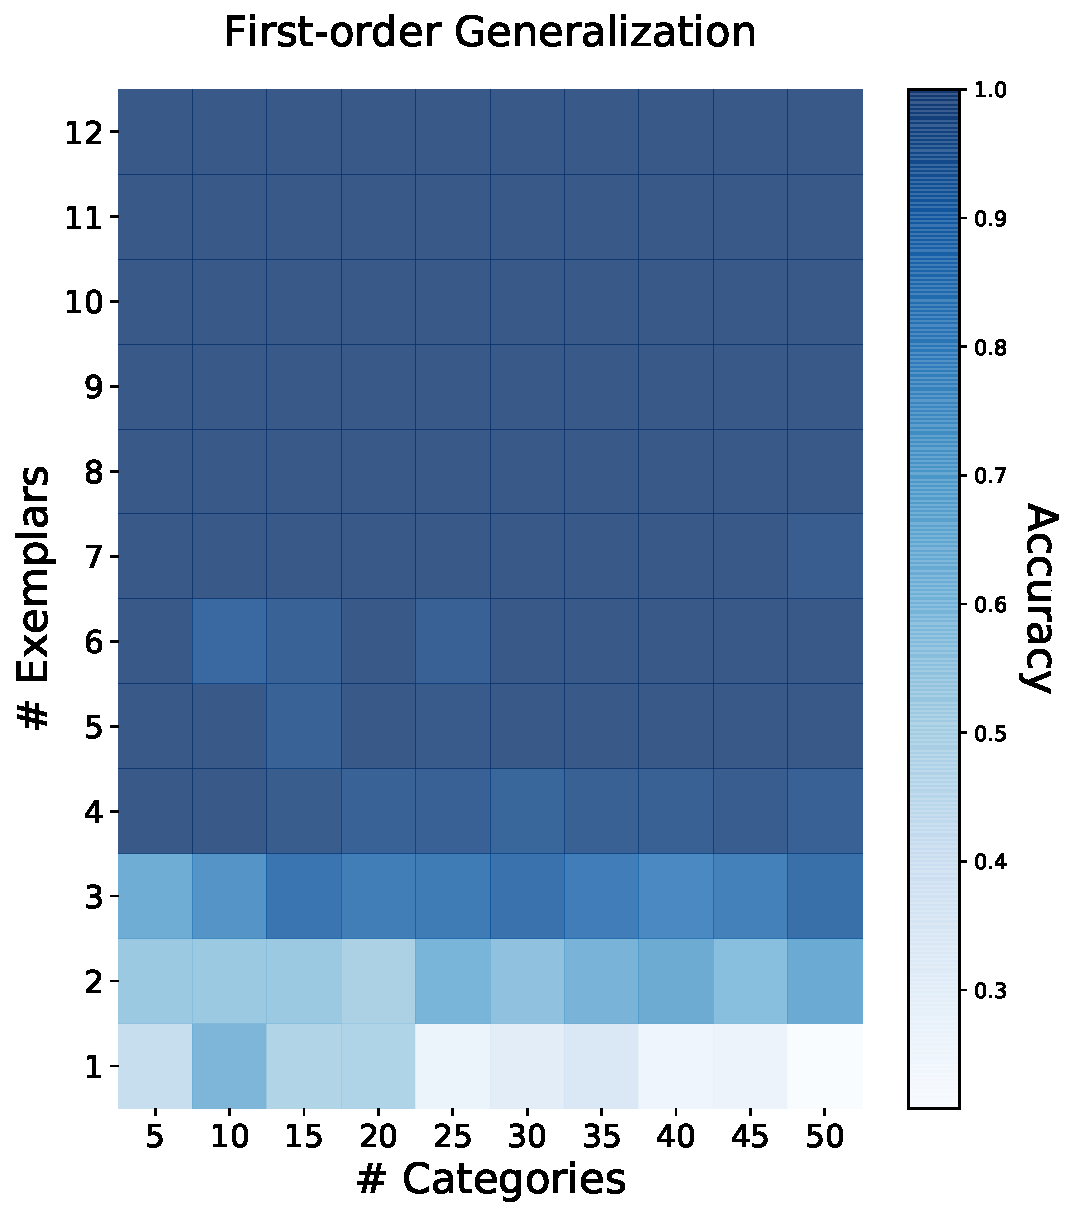
\includegraphics[width=0.98\textwidth]{figures/mlp_1order_accuracy.pdf}
                    \end{center}
                \end{subfigure}
                % subfigure (b)
                \begin{subfigure}[b]{0.48\textwidth}
                    \begin{center}
                        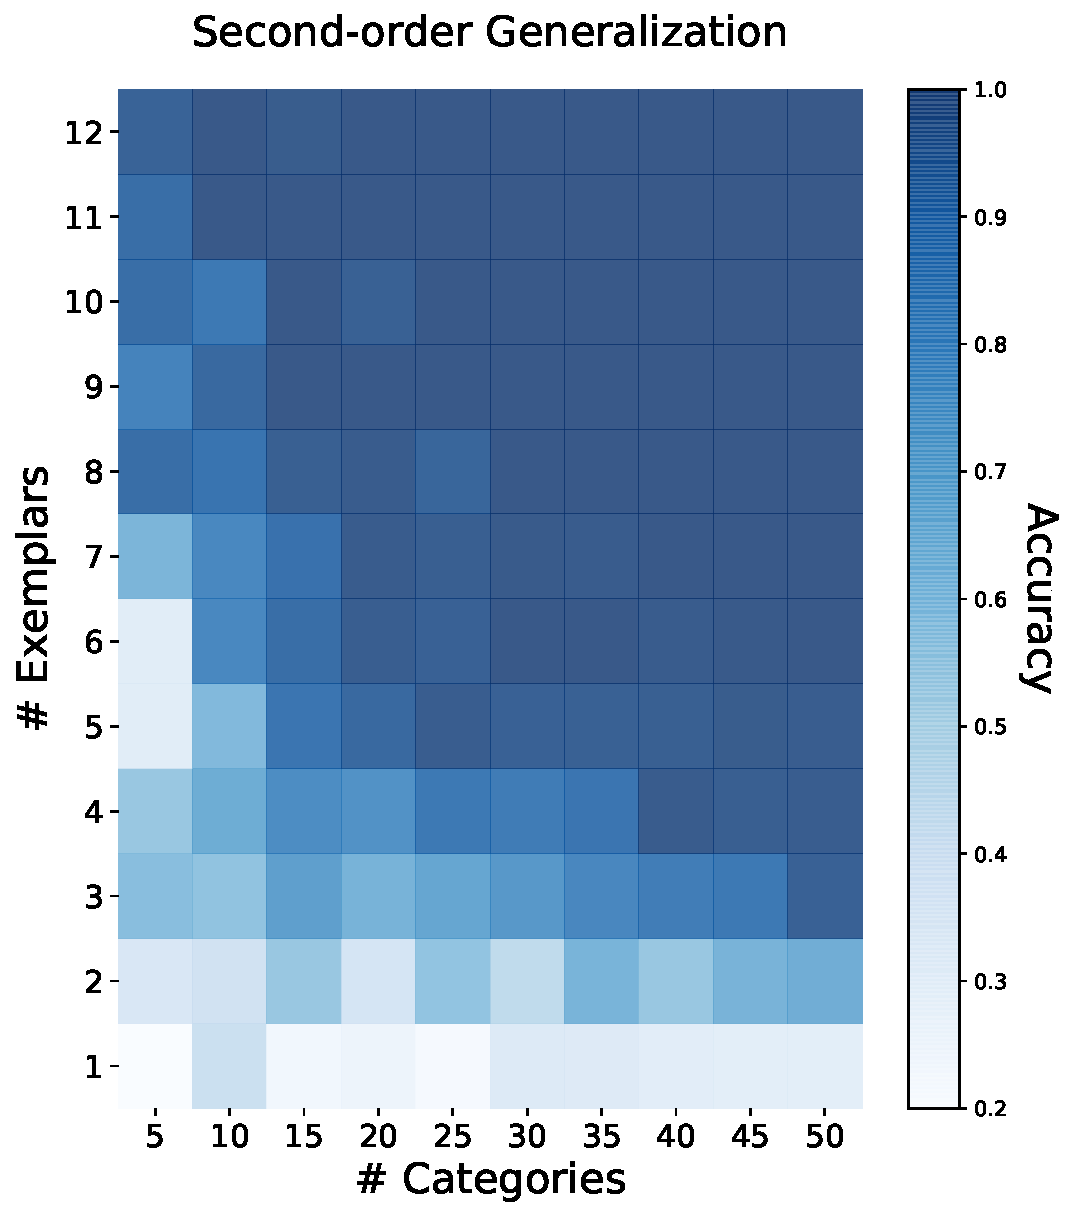
\includegraphics[width=0.98\textwidth]{figures/mlp_2order_accuracy.pdf}
                    \end{center}
                \end{subfigure}
            \end{center}
            \caption{MLP}
            \label{fig:mlp_results}
        \end{subfigure}
        % cnn results
        \begin{subfigure}[b]{0.47\textwidth}
            \begin{center}
                % subfigure (a)
                \begin{subfigure}[b]{0.48\textwidth}
                    \begin{center}
                        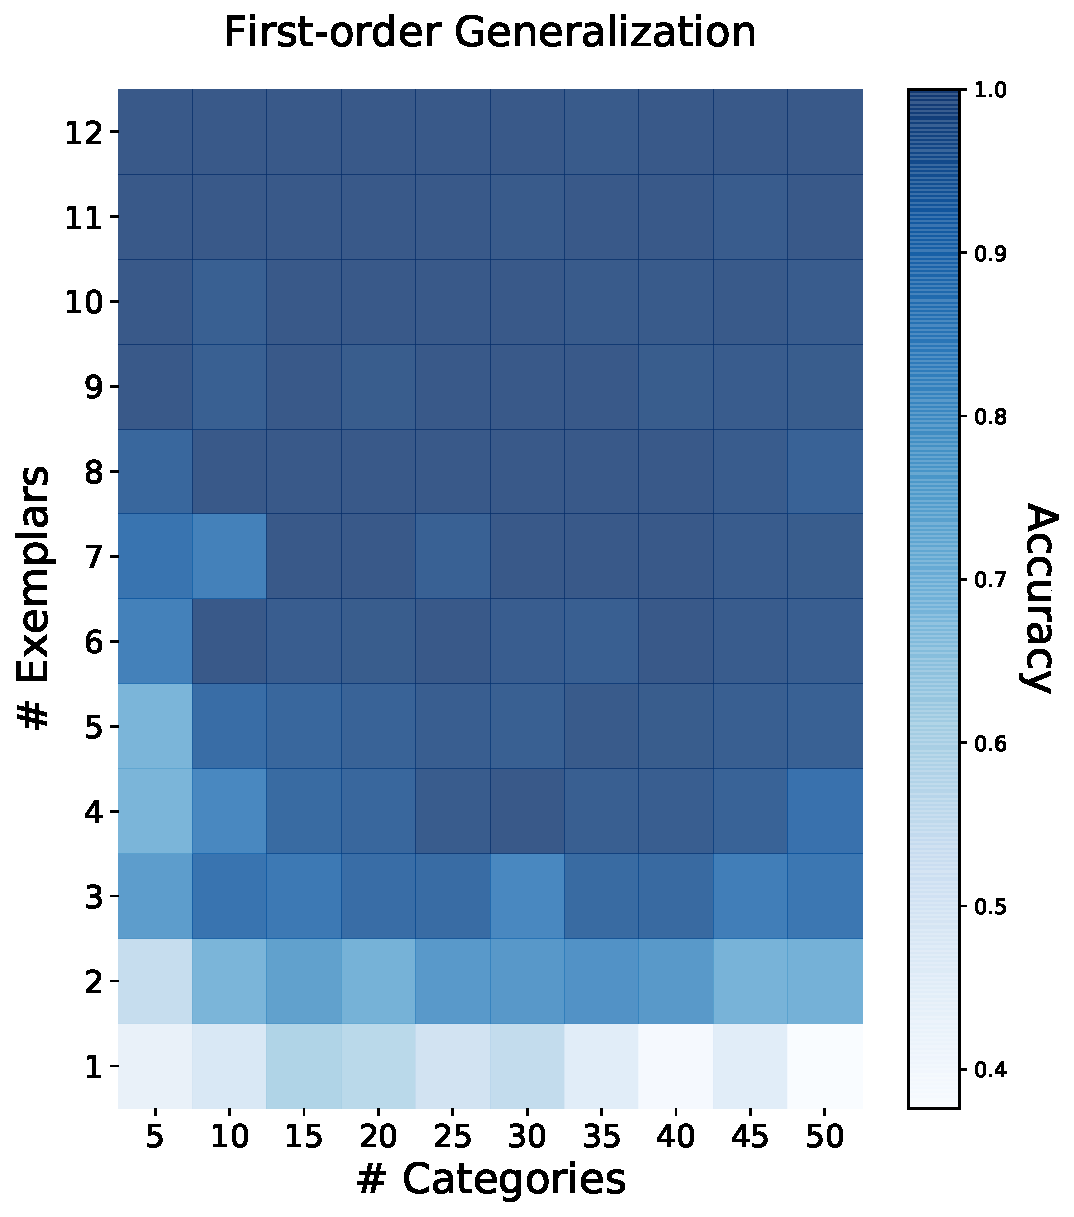
\includegraphics[width=\textwidth]{figures/cnn_1order_accuracy.pdf}
                    \end{center}
                \end{subfigure}
                % subfigure (b)
                \begin{subfigure}[b]{0.48\textwidth}
                    \begin{center}
                        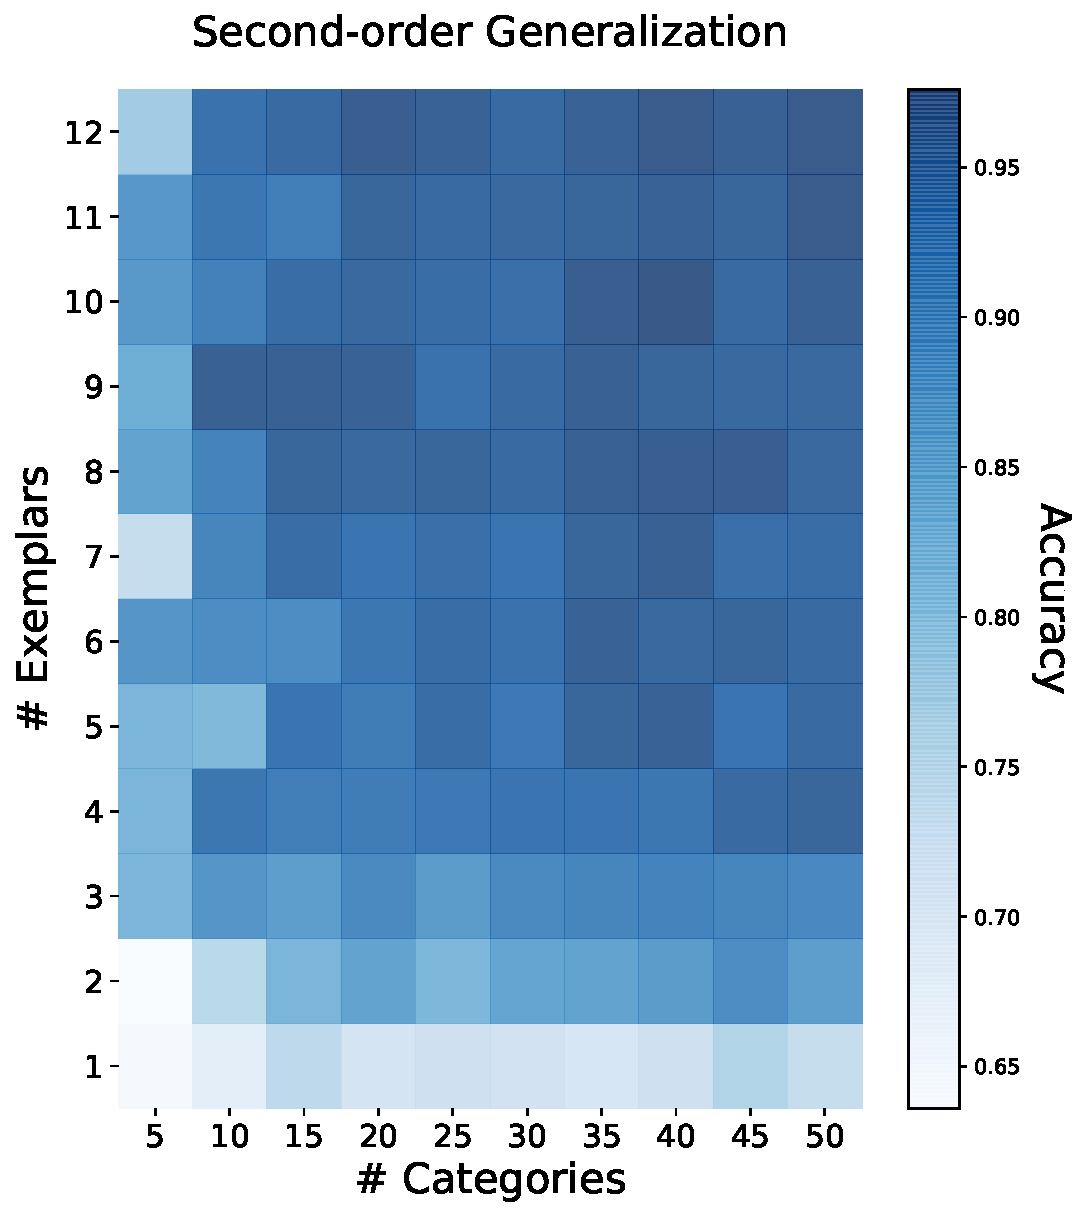
\includegraphics[width=\textwidth]{figures/cnn_2order_accuracy.pdf}
                    \end{center}
                \end{subfigure}
            \end{center}
            \caption{CNN}
            \label{fig:cnn_results}
        \end{subfigure}
    \end{center}
    \caption{First- and second-order generalization results for the simple MLP
    and CNN models. For each \{\textit{\# categories}, \textit{\# exemplars}\}
    pair, the average result from 5 trials is shown.}
    \label{fig:generalization_results}
\end{figure*}